\chapter{付録}	% TODO: 章題を記入．題は任意．
\section{最終セミナーにおける質疑に対する補足解析}
\label{appendix:seminar_response}

本付録では、最終セミナーにおける「今後洋上風車が建設されることで、実際の操業に影響が出ると考えられるか」という質疑に対し、促進区域内に焦点を当てた追加解析の結果を述べる。

本解析では、北海道松前沖に指定された「促進区域」の境界線内に限定して、2024年と2025年の操業海域の重複状況を算出した。図\ref{fig:appendix_union}は、促進区域周辺における漁場の変遷を示したものである。

\begin{figure}[htbp]
  \centering
  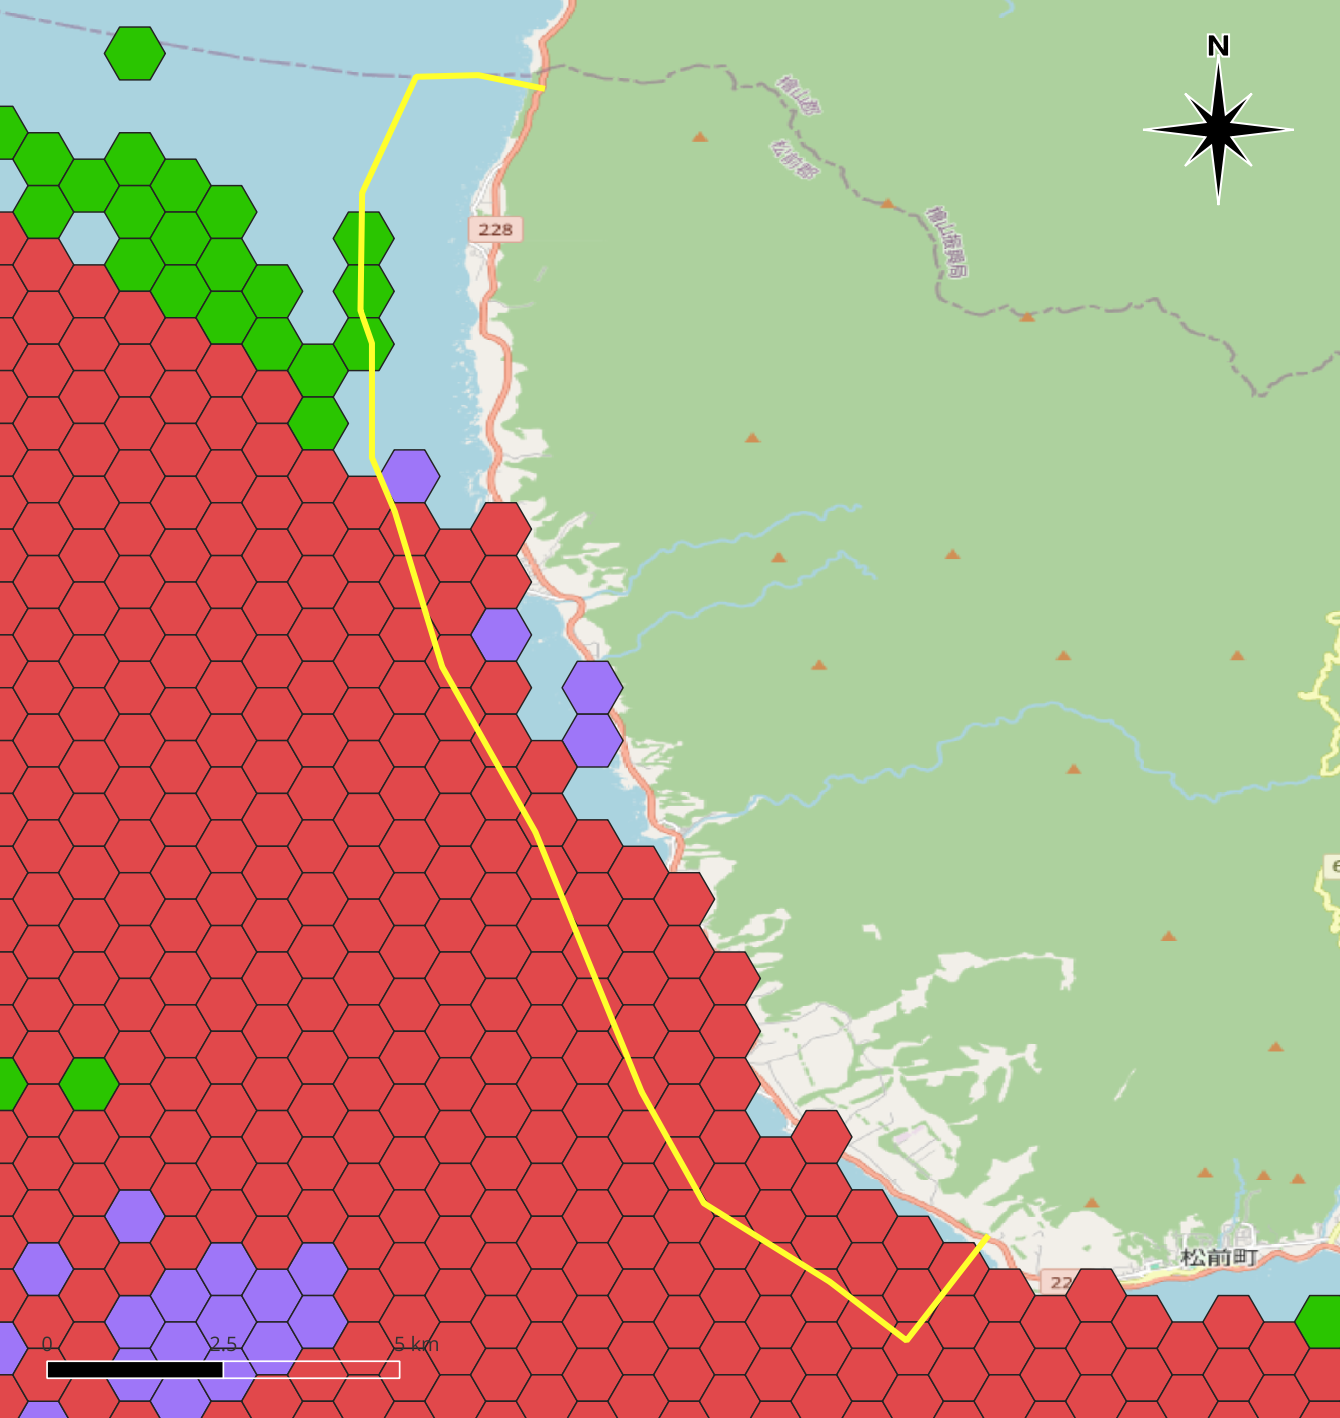
\includegraphics[width=10cm]{images/付録.png}
  \caption{促進区域における漁場利用範囲の比較（赤：共通、緑：2024のみ、紫：2025のみ）}
  \label{fig:appendix_union}
\end{figure}

促進区域内において、2カ年のいずれかで利用が確認されたのは計61グリッドであった。各区分の構成比を表\ref{tab:appendix_stats}に示す。

\begin{table}[htbp]
  \centering
  \caption{促進区域内における利用海域の変遷（2024年・2025年）}
  \label{tab:appendix_stats}
  \begin{tabular}{lrr}
    \hline
    \multicolumn{1}{c}{区分} & \multicolumn{1}{c}{グリッド数 (n)} & \multicolumn{1}{c}{構成比 (\%)} \\
    \hline
    \textbf{共通エリア（赤色）} & \textbf{54} & \textbf{88.5} \\
    2024年のみ利用（緑色） & 3 & 4.9 \\
    2025年のみ利用（紫色） & 4 & 6.6 \\
    \hline
    合計（和集合） & 61 & 100.0 \\
    \hline
  \end{tabular}
\end{table}

解析の結果、促進区域内における両年共通の利用域は、区域内で利用された全海域の88.5\%（54グリッド）に達した。
以上の通り、促進区域内の海域利用は、全域的な解析結果（共通エリア約54\%）と比較して高い重複率を示した。これは、促進区域内の海域利用が年ごとの漁場の変動に左右されにくく、操業において恒常的に利用される海域であることを示唆している。したがって、促進区域への洋上風車建設が実施された場合、年度によらず航路の迂回など、一定の操業影響が継続的に発生する可能性が高いと考えられる。